\section{Introduction}
The effect of spin-orbit and spin-spin interactions were neglected in previous
BNS searches~\cite{Abadie:2011nz}, as they do not have a significant effect on
the $\sim 1600$ gravitational wave cycles in the 40--2000~Hz sensitive band of
first-generation detectors~\cite{Apostolatos:1996rf}. However, aLIGO and AdV
will be sensitive to gravitational-wave frequencies between 10--2000Hz,
increasing the number of cycles in band by an order of magnitude.
Initial studies have demonstrated that over this band, the small secular
effects produced by spin-orbit and spin-spin coupling will have a significant
effect on the detectability of BNS systems with non-trivial component
spins~\cite{Ajith:2011ec}. However, the current geometric method for placing
BNS templates~\cite{Bank06} does not incorporate spin. While numerical
(stochastic) methods could be used to include spin, these require
substantially more templates than a comparable geometric
approach~\cite{Harry:2009ea}. 

We consider two populations of neutron star
binaries: the first has spins uniformly distributed from $\chi = 0$ to $0.4$,
the second, a sub-set of this, has spins between $0$ and $0.05$.  This extended spin
distribution allows for the possibility of serendipitous discovery of BNS
systems in globular clusters, where the evolutionary paths may be different
than that in field binaries~\cite{Grindlay:2005ym}. Since supernova kicks may
cause the direction of the neutron star's angular momentum to be misaligned
with the orbital angular momentum of the binary~\cite{Farr:2011gs}, or the
binaries may be formed by direct capture, we consider  a population of
binaries with an isotropic spin distribution.

We evaluate a new geometric algorithm for placing templates for BNS systems
with spin, presented in \cite{Brown:2012qf},
which has a significantly higher sensitivity than previous
searches. The algorithm constructs a metric on the parameter space using
the various coefficients of the TaylorF2 expansion of the orbital phase as
coordinates. In such a coordinate system the parameter space metric is
globally flat, therefore we can transform into a Euclidean coordinate system.
Finally, our method uses a Principal Coordinate Analysis to identify a two
dimensional manifold that can be used to cover the aligned spin BNS parameter
space using existing two dimensional lattice placement algorithms.

We perform a systematic evaluation of the ability
of a search that neglects spin to detect gravitational waves for BNS in aLIGO
and AdV.  We show that this search will lose more than $3\%$ of the
matched filter signal-to-noise ratio for 59\% (6\%) of signals if it is used to search
for BNS systems with spins uniformly distributed between $0 \le \chi_{1,2} \le
0.4 (0.05)$; this is unsatisfactory over a
large region of the signal parameter space. We show that by considering BNS
systems where the spin of the neutron stars are aligned with the orbital
angular momentum (i.e. the binary is not precessing), we can create a
two-dimensional template bank that is efficient at detecting spin-aligned BNS
signals. Finally we demonstrate that this bank is sufficient to detect signals
from generic spinning, precessing binaries in aLIGO and AdV. The spin-aligned
bank loses more than $3\%$ of the signal-to-noise ratio for only 9\% (0.2\%)
of signals, sufficient to construct a sensitive and unbiased search for BNS
systems in aLIGO and AdV.

\section{BNS Search Sensitivity}
\label{ssec:nonspin_performance}
\label{sec:spin_import}

We quantify the performance of templated matched-filter searches by the
fitting factor (FF) of the search~\cite{Apostolatos:1995pj}.  The fitting
factor is the fraction of the signal-to-noise ratio that would be recovered
when matching a given signal with the best matching waveform in the template
bank. When searching for BNSs, we do not know the exact physical parameters of the
system. We assume that the masses of the neutron stars lie between $1$ and
$3\, M_\odot$ and construct a bank of waveform templates to span this
region of the mass parameter space. We measure the sensitivity of this bank 
using the fitting factor.

In searches for gravitational waves using LIGO and Virgo, the bank is constructed
such that the fitting factor for any signal in the target parameter space will
never be less than 0.97. At least one of the templates in the bank must have a
maximized overlap of 0.97 (or more) with the signal. This value is chosen to
correspond to an event rate loss of no more than 10\% of possible sources
within the range of the detectors~\cite{Cutler:1992tc}. In this chapter, we use
a fitting factor of 0.97 to construct search template banks.

We now test whether a bank of templates that does not model the effect of spin
is sufficient to detect generic, spinning BNS sources in aLIGO and AdV. We
create a bank of non-spinning templates that would recover any
non-spinning BNS system with a fitting factor greater than 0.97.  This bank is
constructed using TaylorF2 waveforms, which are constructed using the stationary
phase approximation to the gravitational-wave phasing accurate to 3.5
post-Newtonian (PN) order~\cite{DPK99,Blanchet:2006zz}. To create a
bank of these waveforms we use the hexagonal-placement method defined in
\cite{Cokelaer:2007kx}, which was used in the majority of previous searches in
LIGO and Virgo~\cite{Abbott:2009tt,Abbott:2009qj,Abadie:2010yba}. This
template bank is placed using the metric given in \cite{OwenSathyaprakash98},
which is valid, by construction, for templates at 2PN order. 
Our signal waveforms are constructed using the SpinTaylorT4
waveform \cite{BCV03b}, a time-domain waveform accurate to 3.5PN order
in the orbital phase which includes the leading order spin-orbit, spin-spin,
and precessional modulation effects and implemented in the LSC Algorithm Library Suite
\cite{lalsuite}. We first confirm that although the
bank is constructed at 2PN order, it yields fitting factors greater than 0.97
for both the TaylorF2 and SpinTaylorT4 non-spinning waveforms at 3.5PN order.
To simulate a population of spinning BNS sources, we generate 100,000 signals
with component masses uniformly distributed between 1 and 3 $M_{\odot}$ and
dimensionless spin magnitudes uniformly distributed between 0 and 0.4. The orientation
of the spin, the orientation of the orbital angular momentum, and the sky
location are isotropically distributed.  To model the sensitivity of a second
generation gravitational wave interferometer, we use the aLIGO zero-detuned,
high-power sensitivity curve \cite{aLIGOSensCurves}. For our simulations, we
use a lower frequency cutoff of 15Hz.

We note that for non-precessing systems
the fitting factor is independent of the detector alignment and location; however
this statement is not true for precessing systems. For such systems, however,
the distribution of fitting factors over
a population of sources will be independent of the detector alignment
and location. Therefore, for this study we calculate the fitting-factor for a single
detector with an arbitrary location and position.

%we
%investigate how our conclusions are affected if a 10Hz lower frequency cut-off
%is used or if the Advanced Virgo noise PSD \cite{aVirgo,advvirgowebsite}
%is used in section \ref{ssec:other_noise_curves}.

In Fig.~\ref{fig:no_spin_cover} we show the distribution of fitting factors
obtained when searching for our population of BNS sources with the
non-spinning template bank. We see that 59\% of signals were recovered with a
fitting factor less than 0.97.  If the maximum spin magnitude is restricted to
0.05, we find that 6\% of signals are recovered with a FF less
than 0.97.  If BNS systems do exist with spin magnitudes up to 0.4, a template
bank that captures the effects of spin will be required to maximize the number
of BNS detections.  Detection efficiency will be greatly reduced by using a
template bank that only contains waveforms with no spin effects.  Even under
the assumption that component spins in BNS systems will be no greater
than 0.05, detection efficiency will be decreased if the effect of spin on the
signal waveform is ignored.

\begin{figure}
\begin{center}
\includegraphics[width=1.0\textwidth]{papers/bns_spin/figure1.pdf}
\end{center}
\caption{\label{fig:no_spin_cover} The distribution of fitting factors obtained by searching
for the precessing BNS systems described in section \ref{ssec:nonspin_performance}
with component spins up to 0.4 (blue solid line), 0.2 (green dashed line), and 0.05 (red dotted line) using the non-spinning
BNS template bank described in section \ref{ssec:nonspin_performance} and the advanced LIGO, zero-detuned,
high-power PSD with a 15Hz lower frequency cutoff.}
\end{figure}

\section{A template placement algorithm for aligned-spin BNS templates}
\label{sec:param_space}

As we have demonstrated in the previous section, there is a substantial region
of the BNS parameter space where a significant loss in signal-to-noise ratio
would be encountered when searching for astrophysically plausible, spinning
BNS systems with non-spinning templates. It has been suggested that using BNS
templates where the spins of the system are aligned with the orbital angular
momentum is sufficient for detecting generic BNS systems with second-generation
detectors~\cite{Ajith:2011ec} using TaylorF2 templates that incorporate the
leading order spin-orbit and spin-spin corrections~\cite{PW95}. 

In this section we use these spin-aligned waveforms to construct a template
bank that attempts to cover the full space of astrophysically plausible BNS
spin configurations. This template bank should contain as few templates as
possible, while still being able to detect any BNS system that might be
observed with aLIGO and AdV. We use TaylorF2
waveforms accurate to 3.5PN order in orbital phase and including the
leading order spin-orbit and spin-spin terms given by~\cite{PW95,Buonanno:2009zt}
Since BNS systems coalesce at $\sim 1500$~Hz, significantly higher than the
most sensitive band of the detectors, the waveform will be dominated by the
inspiral part of the signal~\cite{Buonanno:2009zt}.  The effect of component
spin on BNS inspiral waveforms has been well explored in the
literature~\cite{Apostolatos:1994mx,Kidder:1992fr,Kidder:1995zr,BCV03b}).
%Compared to non-spinning BNS systems, the phase evolution of an aligned-spin
%BNS system is affected by additional terms due to the presence of spin.
For spin-aligned (i.e. non-precessing) waveforms, the dominant effects of
component spin are spin-orbit coupling, which enters the waveform phasing at
1.5PN order, and spin1-spin2 coupling, which enters the waveform phasing at
2PN order.  Other spin-related corrections to the PN phasing have been
computed \cite{Mikoczi:2005dn,Arun:2008kb}, however, in this work we mainly restrict
to only the two dominant terms. 

Based on the results of \cite{Brown:2012qf}, where we derive a metric for
aligned-spin TaylorF2 waveforms, we can use a geometric algorithm for template
bank placment. We place a hexagonal grid of templates
in the two dominant coordinates $\xi_1$, $\xi_2$, which are derived
in \cite{Brown:2012qf}. For BNS systems in aLIGO 
and AdV the extent of the physical parameter
space in the remaining directions is smaller
than the coverage radius of a template and can be neglected in nearly the entire parameter space.
As the effective dimension  of the space is two-dimensional, a
hexagonal placement algorithm, similar to that used in previous searches of
LIGO and Virgo data, can be employed to cover the space. This allows the
method to be incorporated into existing search pipelines in a straightforward
way. Where the third dimension, $\xi_3$, cannot be neglected, we stack the templates
to ensure that the maximum mismatch due to the depth than 0.25\%.
For an aligned-spin template bank where the spin of each component is restricted to 0.4,
using the advanced LIGO, zero-detuned high-power noise curve with a lower frequency cut-off of 15Hz,
we find that approximately 520,000 templates are required.
Roughly 100,000 of these templates were added by the stacking process.

% Compare non-spinning component to full spin
We can verify that the template bank algorithm is working correctly by repeating the simulation described
in section \ref{ssec:nonspin_performance}, but evaluating the fitting factor between our bank of aligned-spin
template waveforms and a set of signals that is restricted to having spins that are (anti-)aligned with the
orbital angular momentum. The results of this simulation are shown in figure \ref{fig:anstar-aligned} and
one can see that with our bank we do not observe fitting factors lower than 0.97 when searching for aligned
spin BNS systems.

\begin{figure}
\begin{center}
\includegraphics[width=1.0\textwidth]{papers/bns_spin/figure5.pdf}
\end{center}
\caption{\label{fig:anstar-aligned} The distribution of fitting factors obtained by searching
for aligned spin, binary neutron star systems, with spin magnitudes restricted to 0.4
using the aligned-spin BNS template bank described in section \ref{sec:param_space}
and the aLIGO, zero-detuned, high-power PSD with a 15Hz lower frequency cutoff.}
\end{figure}

In the previous paragraphs we have restricted attention to the aLIGO
zero-detuned, high-power predicted sensitivity with a 15Hz lower frequency cut off. However,
we should verify that the conclusions we have drawn are valid for AdV, whose
PSD is different from that of aLIGO, as shown in Figure \ref{fig:asd_comparison}. Additionally we
should also show that the choice to use a 15Hz cut off in the aLIGO PSD does not affect
the conclusions made in this section. Using our method we find that we require approximately 120,000 templates to cover the
parameter space for AdV, in comparison to approximately 520,000 templates for aLIGO. By comparing the results when using the aLIGO PSD with a 10Hz and 15Hz lower cut off we observe
that using a 10Hz lower frequency cut off will increase the number of necessary templates from $\sim520000$
to $\sim860000$. 

\begin{figure}
\begin{center}
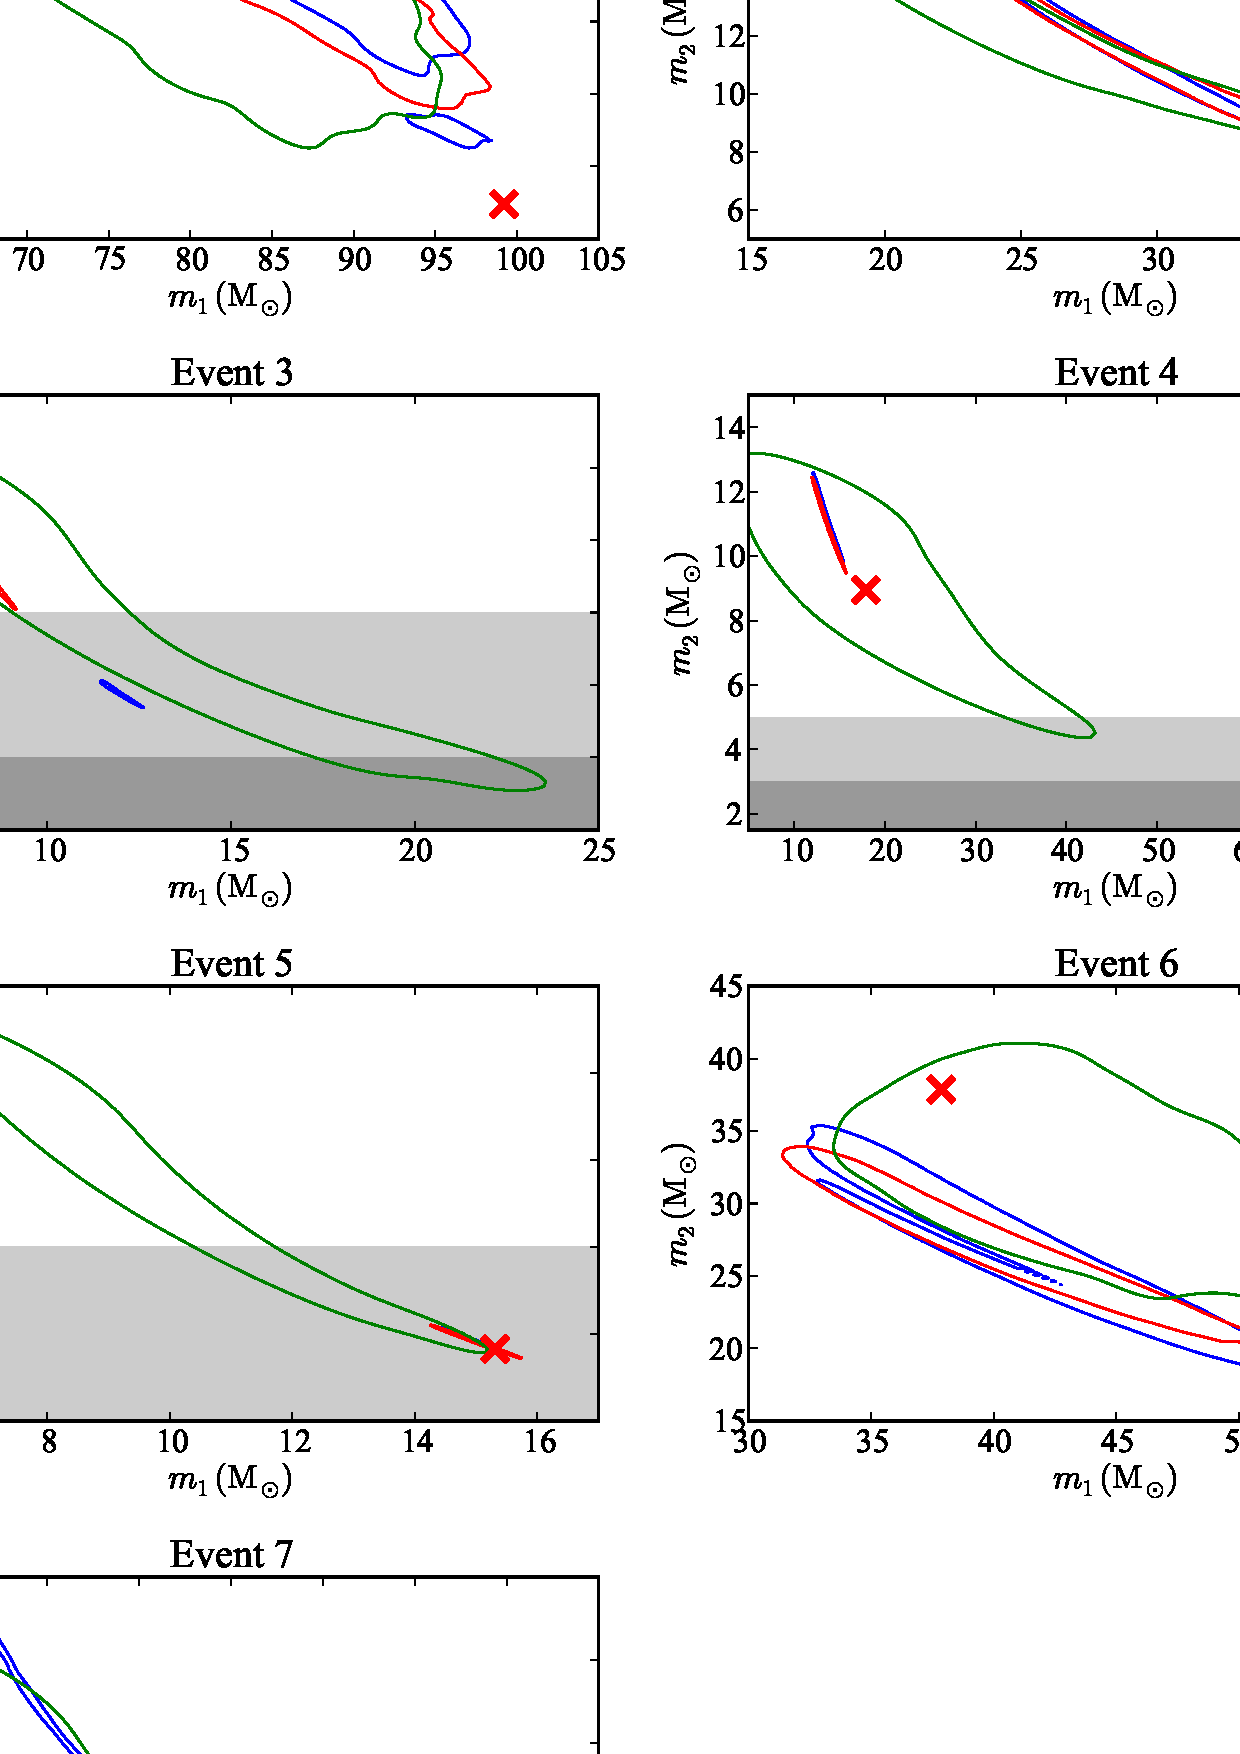
\includegraphics[width=1.0\textwidth]{papers/bns_spin/figure6.pdf}
\end{center}
\caption{\label{fig:asd_comparison} The amplitude spectral density for the aLIGO
zero-detuned high-power design sensitivity (blue solid curve), AdV design sensitivity
(red dashed curve), initial LIGO design sensitivity (blue bot-dash curve) and initial
Virgo design sensitivity (red dotted curve).}
\end{figure}

\section{Comparison to alternative placement methods}

An alternative approach to template placement for aligned spin systems is to use templates
with ``unphysical'' values of the symmetric mass ratio, $\eta$.
That is, to use non-spinning templates, with the desired range of chirp
mass but where the range of $\eta$ values is extended to include both values of $\eta$ that are much lower than
the relevant parameter space and values of $\eta$ that are much higher,
including templates with $\eta$ greater than the physically possible limit of 0.25.

While unphysical $\eta$ templates will produce an increase in efficiency when compared with non-spinning templates, the
method is not as efficient as the aligned spin geometrical placement we have described. In addition, both methods
require the same number of templates to cover the parameter space. Therefore, we would recommend using aligned spin templates
placed using our metric algorithm as opposed to unphysical $\eta$ templates.

Finally, we wish to compare the performance of the geometrical algorithm with the stochastic bank proposed in
\cite{Harry:2009ea,Babak:2008rb}. The stochastic placement works by randomly placing points within the parameter
space and rejecting points that are too ``close'' to points already in the bank. This
has the advantage that it is valid for any parameter space metric, so we could use any of the metrics discussed
above. 

The disadvantage to a stochastic bank, when compared to a geometrically placed bank, is that it will require more
templates to achieve the same level of coverage \cite{Harry:2009ea,Manca:2009xw}.
For our parameter space, consisting of BNS signals with
component spins up to 0.4 and using the advanced LIGO zero-detuned high-power design curve with a 15Hz lower
frequency cut-off, we found that the stochastic placement
produced a bank containing $\sim 750000$ templates, which is 44\% more than with the geometrical placement.
However, stochastic placement can still be used to place templates when no analytical metric is known, such
as when the merger becomes important. In such regions of parameter space, the stochastic placement may still be the best
algorithm to use to place a template bank.

\section{Performance of the aligned spin template bank}
\label{sec:aligned_spin_performance}

In this section we would like to investigate the improvement in the 
detection of generic BNS systems that results from using a template bank
that includes the dominant, non-precessing, spin effects. To do this we use the aligned spinning bank that
we detail in section \ref{sec:param_space} and compare this to the results of using a nonspinning bank 
as shown in section \ref{sec:spin_import}. 

Using our aligned spin template bank, we repeat the investigation from section \ref{sec:spin_import}. We create a 
population of source BNS signals identical to those used in \ref{ssec:nonspin_performance}, and compute the fitting factor
between these signals and the aligned spin template bank. The results of this are shown in FIG.\ref{fig:anstar-prec}.
To decrease the computational cost of this test, we only calculated the overlaps between a signal and templates that
were within a range of $\pm0.1M_{\odot}$ in chirp mass. This is reasonable because the overlap will decrease rapidly
with small changes in chirp mass,
therefore we expect templates with very different values of chirp mass to have low overlaps with each other. We verified
that this approach did not cause us to underestimate the fitting-factor of our banks.

We can now compare the results obtained in this section, using our aligned-spin template bank, with the results obtained in section
\ref{sec:spin_import}, using a non-spinning template bank. One can clearly see an 
improvement in the distribution of fitting factors when using the aligned spin template bank. The fraction
of signals that fall below a fitting factor of 0.97, when the spin magnitudes are restricted to 0.4, falls from 59\% to 9\%.
We also see an  improvement for signals that have spin magnitudes restricted to 0.05, where the fraction of signals falling below a
fitting factor of 0.97 drops from 6\% to 0.2\%. We can also compare the performance of the aligned-spin bank to that of the
non-spinning bank as a function of the maximum spin magnitude,
as shown in Figure \ref{fig:anstar-st-spin}. From this Figure we can see that regardless of the maximum component
spin, the aligned spin bank will greatly reduce the number of signals recovered with fitting factors less than 0.97.

\begin{figure}
\begin{center}
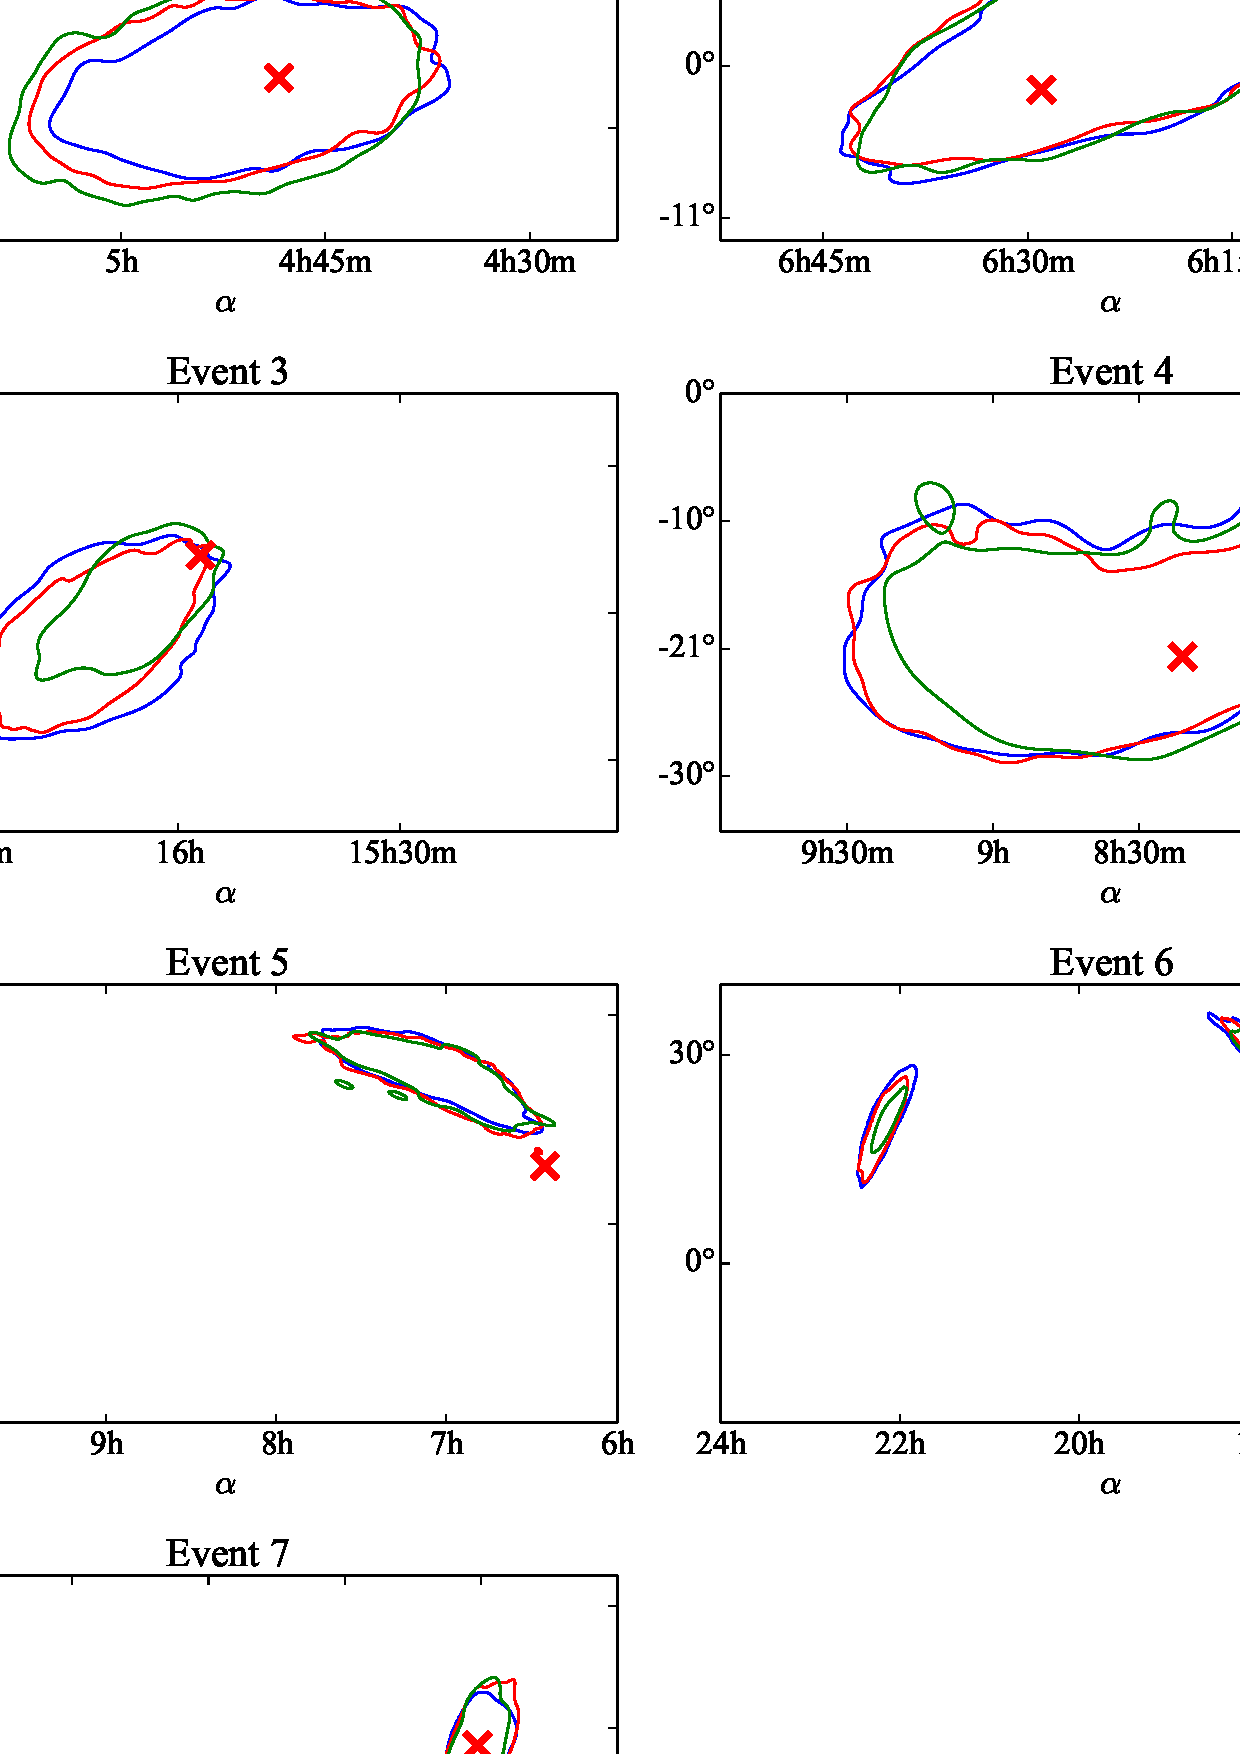
\includegraphics[width=1.0\textwidth]{papers/bns_spin/figure10.pdf}
\end{center}
\caption{\label{fig:anstar-prec} The distribution of fitting factors obtained by searching
for the precessing signals described in section \ref{ssec:nonspin_performance}
with component spins up to 0.4 (blue solid line), 0.2 (green dashed line), and 0.05 (red dotted line) using the aligned spin
BNS template bank described in section \ref{sec:param_space} and the advanced LIGO, zero-detuned,
high-power PSD with a 15Hz lower frequency cutoff.}
\end{figure}
% We want to answer: 
% Does the aligned spin work as designed? 
% How well does it work for generic BNS systems?
\begin{figure}
\begin{center}
\includegraphics[width=1.0\textwidth]{papers/bns_spin/figure11.pdf}
\end{center}
\caption{\label{fig:anstar-st-spin} The fraction of the precessing signals described in
section \ref{ssec:nonspin_performance} recovered with a fitting factor less than 0.97 as
a function of the maximum component spin. Shown for the non-spinning
BNS template bank described in section \ref{ssec:nonspin_performance} (blue solid line),
and the aligned spin
BNS template bank described in section \ref{sec:param_space} (red dotted line). The advanced LIGO, zero-detuned,
high-power PSD with a 15Hz lower frequency cutoff was used when computing the fitting factors.}
\end{figure}

A small fraction of signals fall below a FF of 0.97, even when using the new aligned-spin template bank.
We expect that these poor matches with the aligned template bank are
due to precession. In general, precessional effects will not be important in BNS systems
as the orbital angular momentum is significantly larger than the component spins.
In such cases there is only a small angle between the total and orbital angular momenta
and precession has only a small effect on the waveform.

However, there is a small region of parameter space where precessional effects \textit{will}
have an effect for BNS systems.
Using the model of Ref.~\cite{Brown:2012gs}, applied to the small precession angles in BNS systems, 
we can predict for which systems precession will be most important.
The orientation of a precessing binary must be defined using the total angular momentum rather than the 
orbital angular momentum as done with non-precessing binaries. 
The orientations with the worst matches should be those where the system is edge-on 
(angular momentum perpendicular to the viewing direction) and where the detector is nearly insensitive 
to the plus polarization and only sees the cross polarization (a binary overhead of the detector would have 
its angular momentum oriented $45^{\circ}$ between the arms of the detector).
We find that
this is indeed the case; in fact, all cases with fitting factors less than 0.95 are close to
this configuration. All of these cases also have biases in the recovered mass and
spin parameters due to the secular effects of precession on the phasing of the waveform.

\section{Conclusions}

In this work we have investigated the effects of neglecting spin when
searching for binary neutron star systems in aLIGO and AdV. We have found
that, if component spins in binary neutron star systems are as large as 0.4,
then neutron star spin cannot be neglected, and there is a non-trivial loss in
signal-to-noise ratio even if the maximum spin is restricted to be less than
0.05. We have shown that the
geometric algorithm for placing and aligned spin template bank works for
aligned spin systems and have demonstrated that it does significantly better
for generic, precessing BNS systems than the traditional non-spinning bank.
However, for the BNS aligned spin $\chi_i < 0.4$ parameter space the aligned
spin bank requires approximately five times as many templates as the
non-spinning bank. This increased number of templates will increase the
computational cost of the search and increase the number of background events,
so needs to be balanced against the potential gain in being able to cover a
larger region of parameter space. A further advantage of this method is the ease
with which it can be incorporated into existing or future search
pipelines, which include the use of signal-based vetoes~\cite{Allen:2004gu}
and coincidence algorithms~\cite{Robinson:2008}. In future work we will
investigate how this template bank performs in data from the aLIGO and AdV
detectors which includes non-Gaussian and non-stationary noise features.
Finally we note that the method proposed in this work should be applicable
wherever the TaylorF2 waveforms closely represent actual gravitational
waveforms. In a future work we will investigate how well this method performs
in the binary black hole and neutron-star, black-hole regions of the parameter space.
Wherever the TaylorF2 approximation begins to break down, a stochastic
bank placement may still be the most viable option.
